%第3-3章
\section{基本設計}
基本設計では、ひとまとまりの処理の内容の流れを表現するために用いるアクティビティ図を作成し、「室内環境を監視する(図\ref{a_kansi})」、「換気要請の受け取り(図\ref{a_kanki})」、「入室危険度の確認(図\ref{a_nyuusitu})」、「室内環境状態の表示(図\ref{a_situnaikankyou})」の4つのユースケースについて、簡単に処理の流れを確認した。以下に作成したアクティビティ図を示す。


\begin{figure}[H]
	\centering
	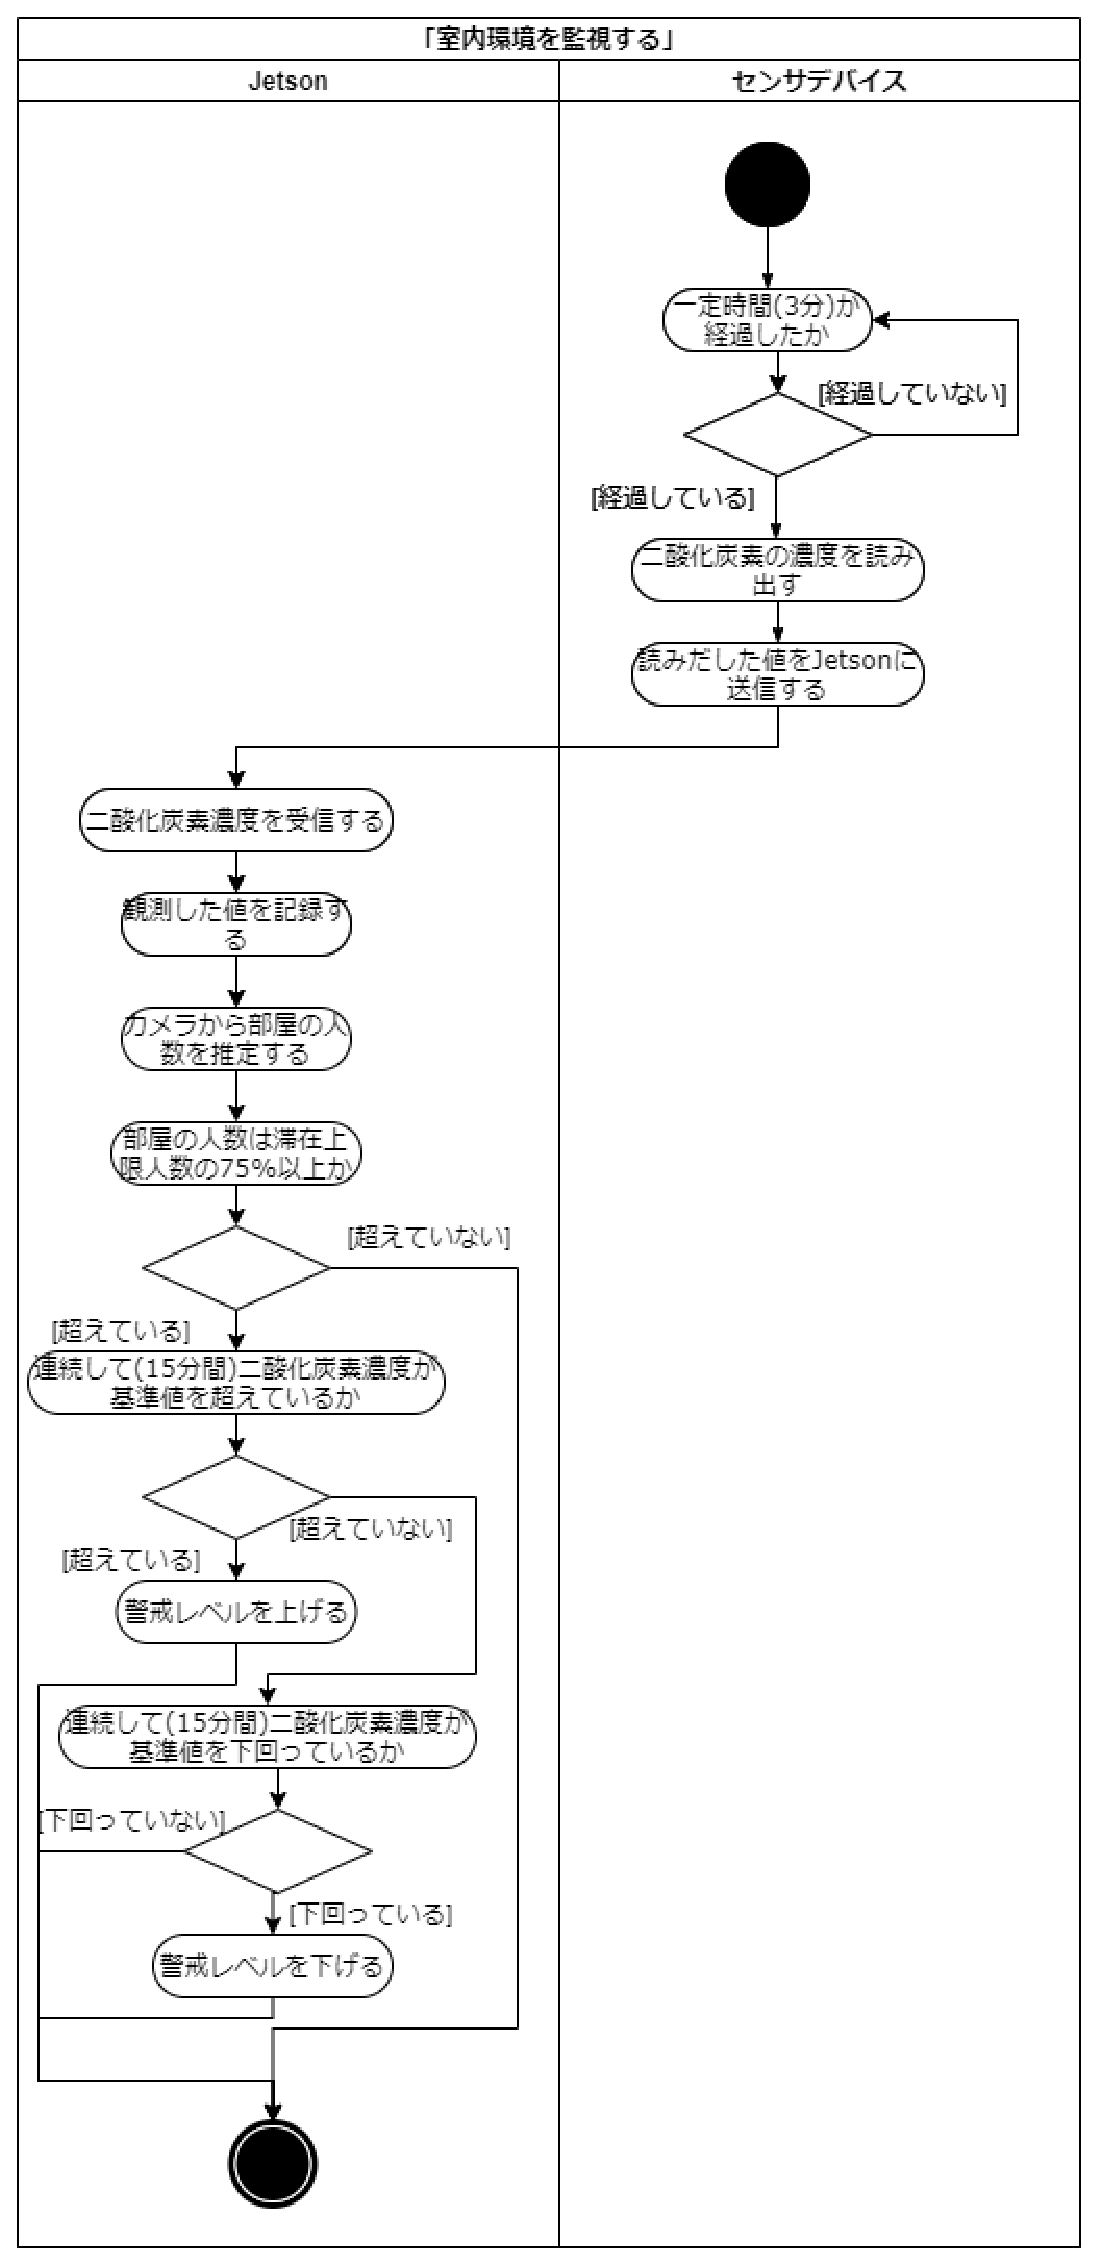
\includegraphics[width=9.5cm]{a_kansi.eps}
	\caption{室内環境を監視する}
	\label{a_kansi}
\end{figure}

\begin{figure}[H]
	\centering
	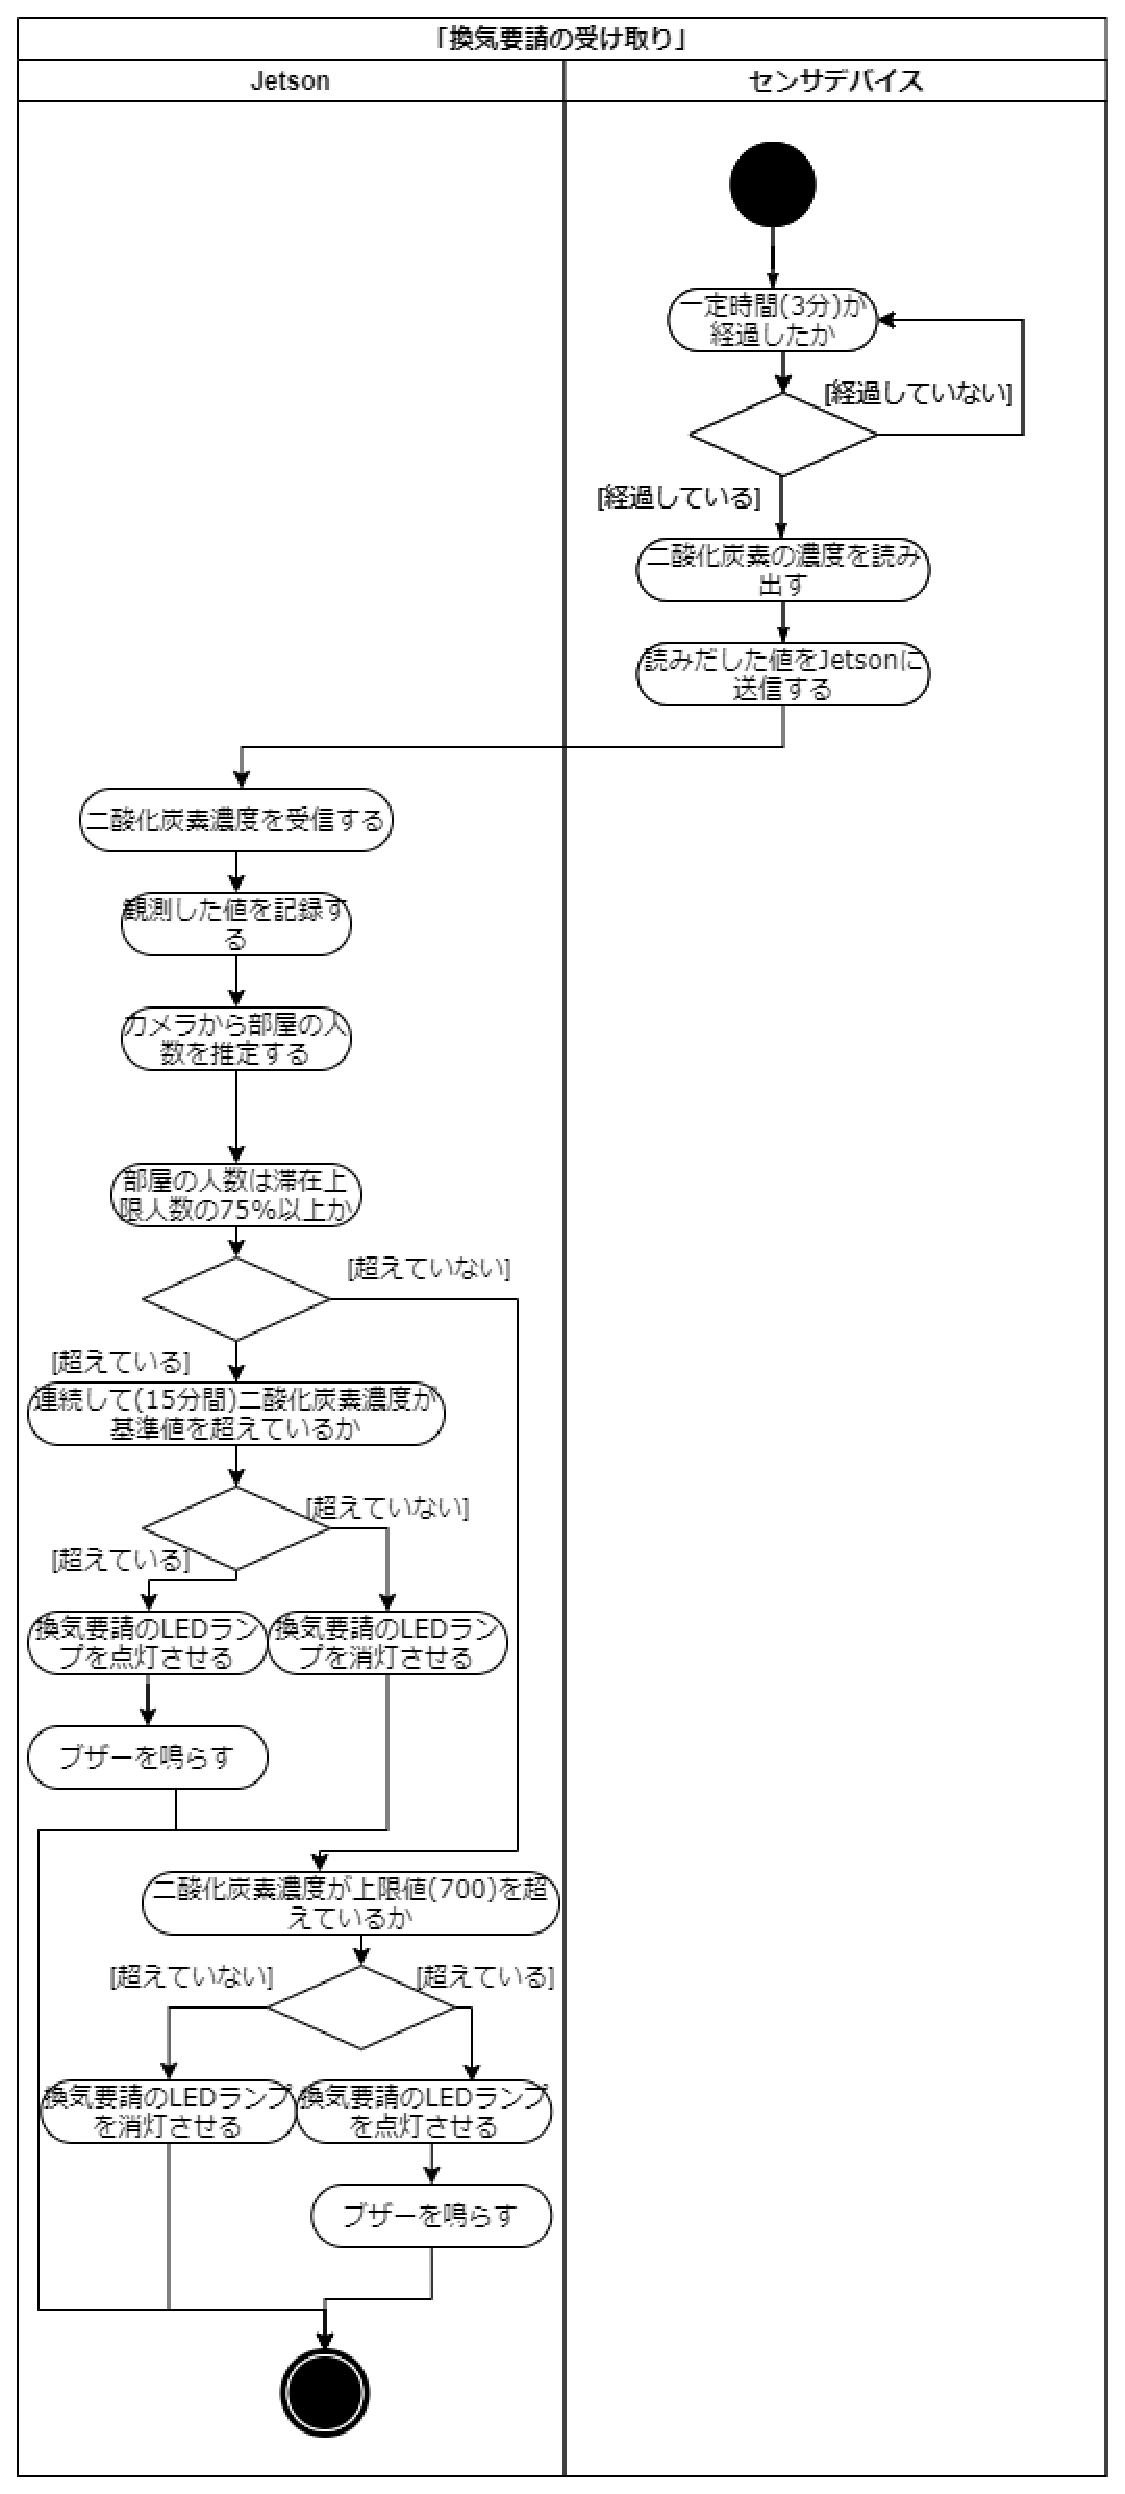
\includegraphics[width=9.0cm]{a_kanki.eps}
	\caption{換気要請の受け取り}
	\label{a_kanki}
\end{figure}

\begin{figure}[H]
	\centering
	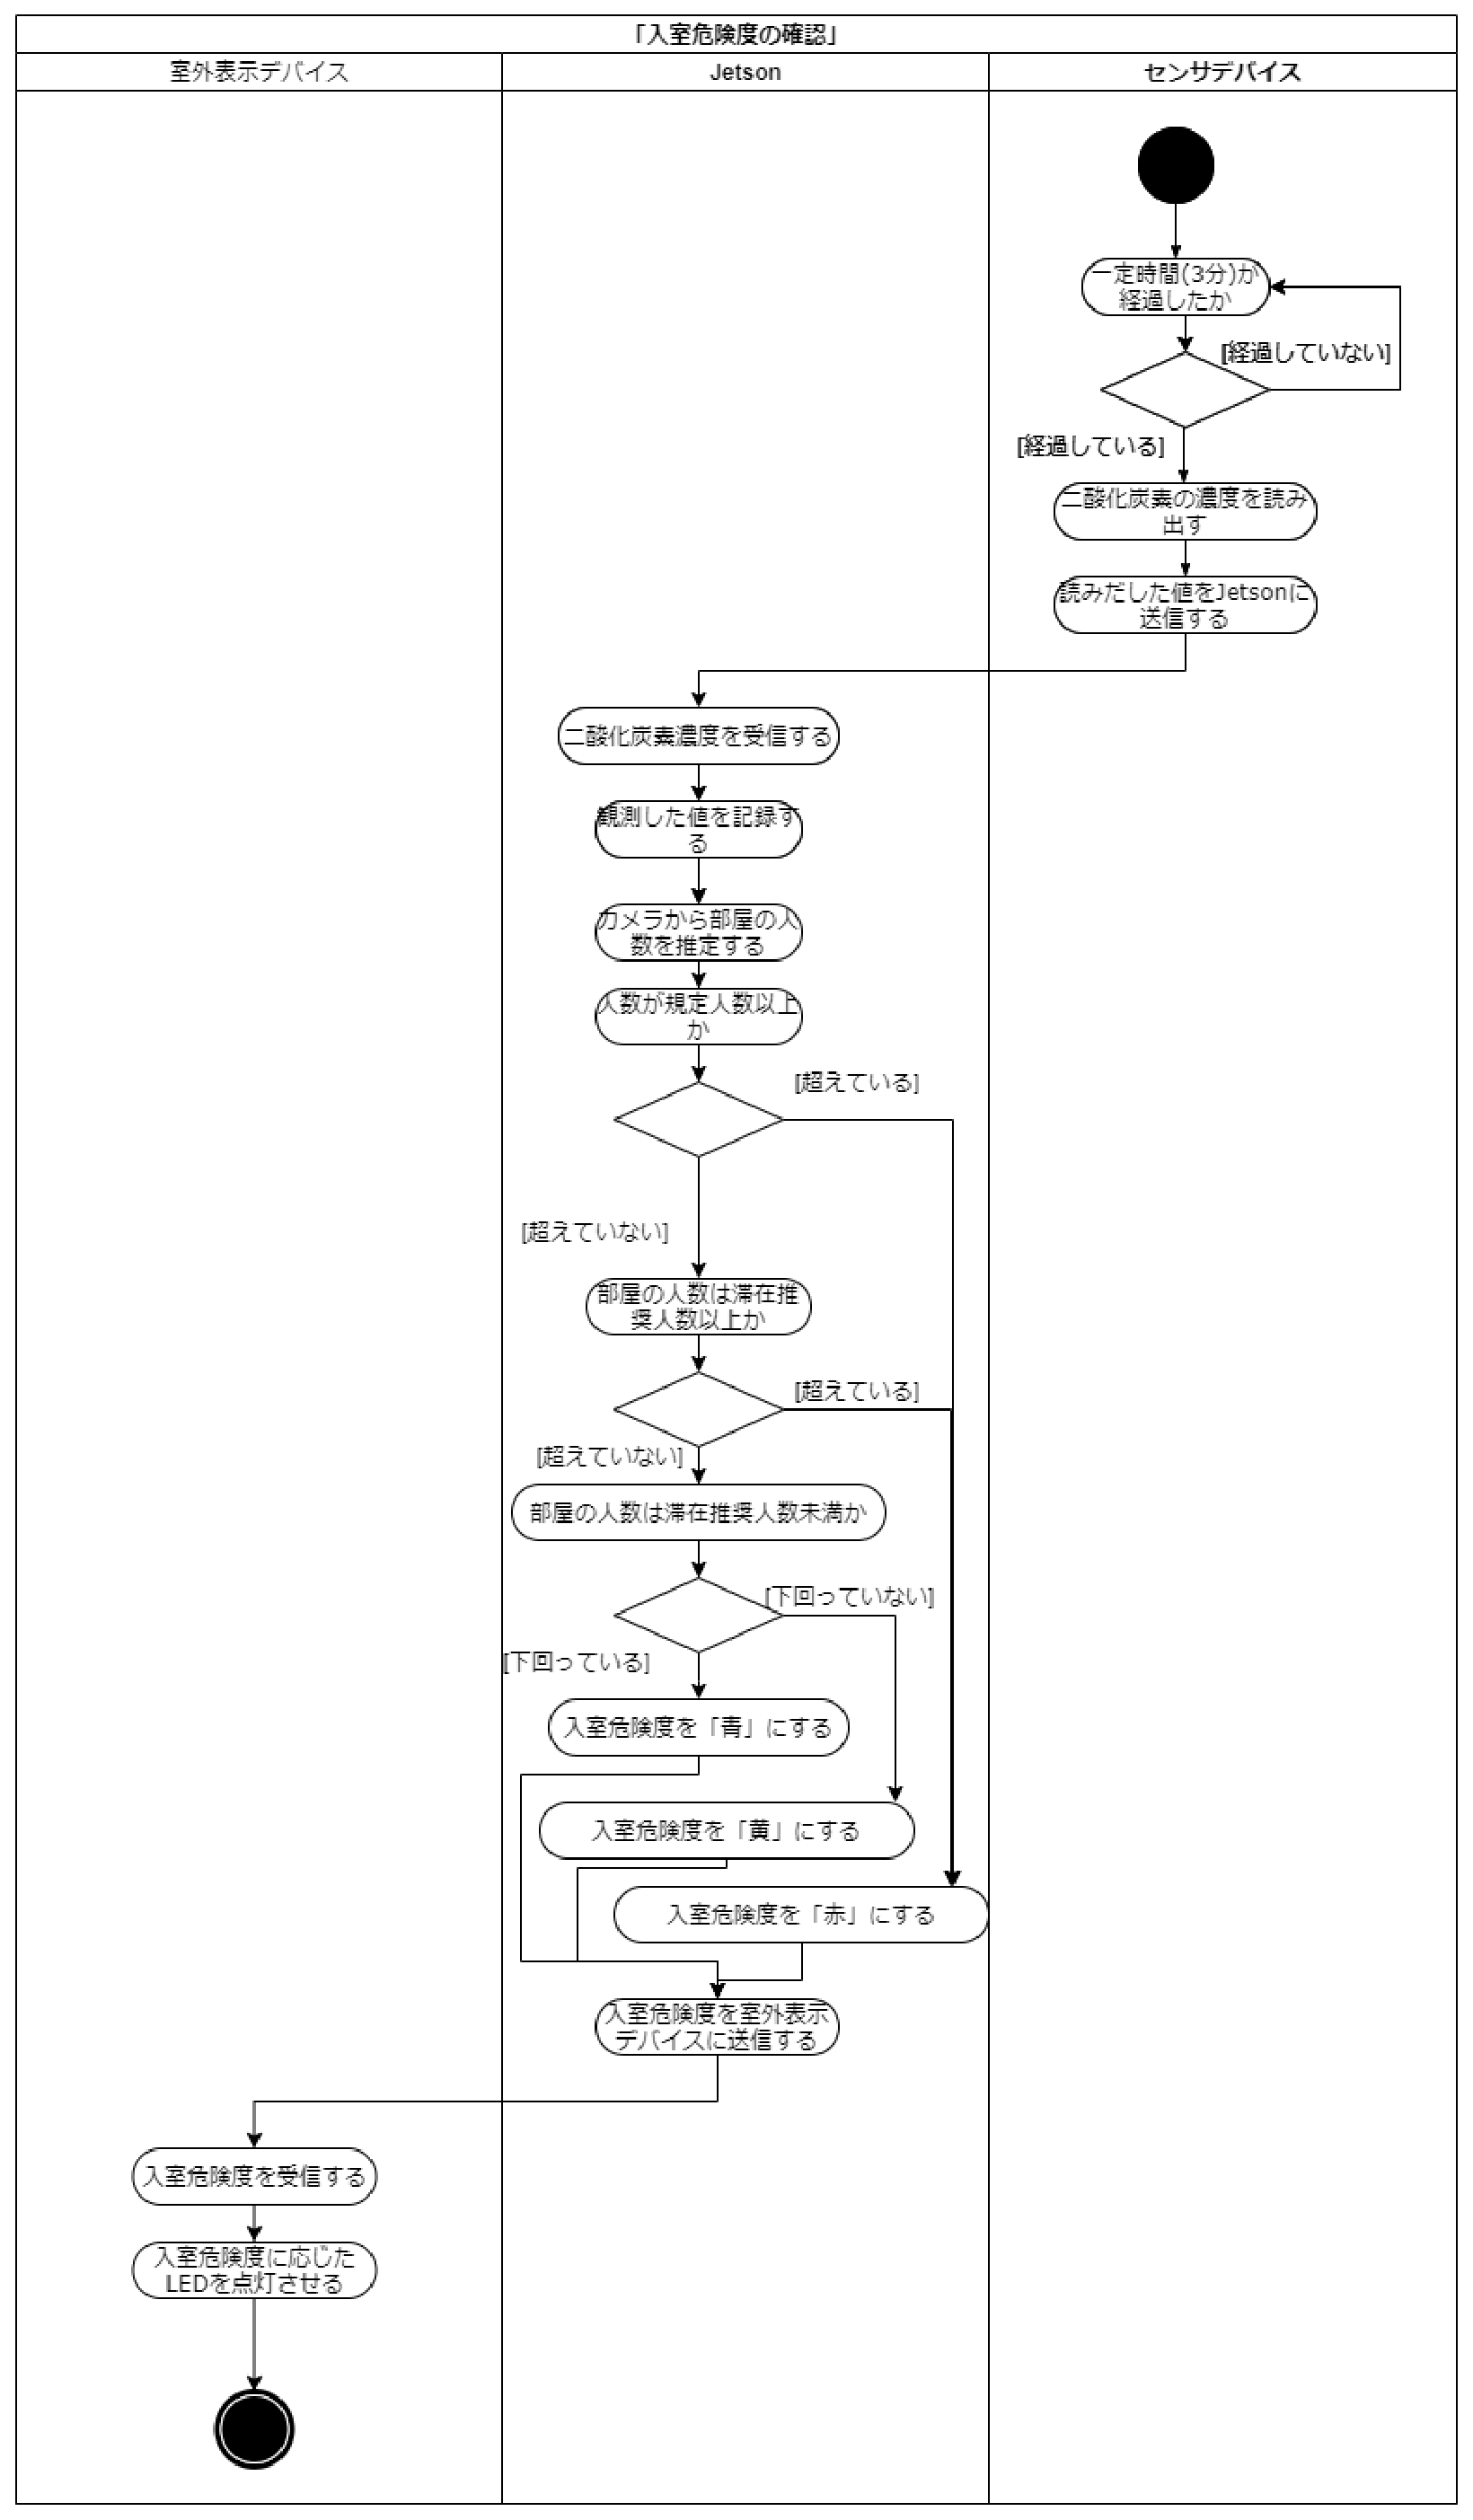
\includegraphics[width=9.5cm]{a_nyuusitu.eps}
	\caption{入室危険度の確認}
	\label{a_nyuusitu}
\end{figure}

\begin{figure}[H]
	\centering
	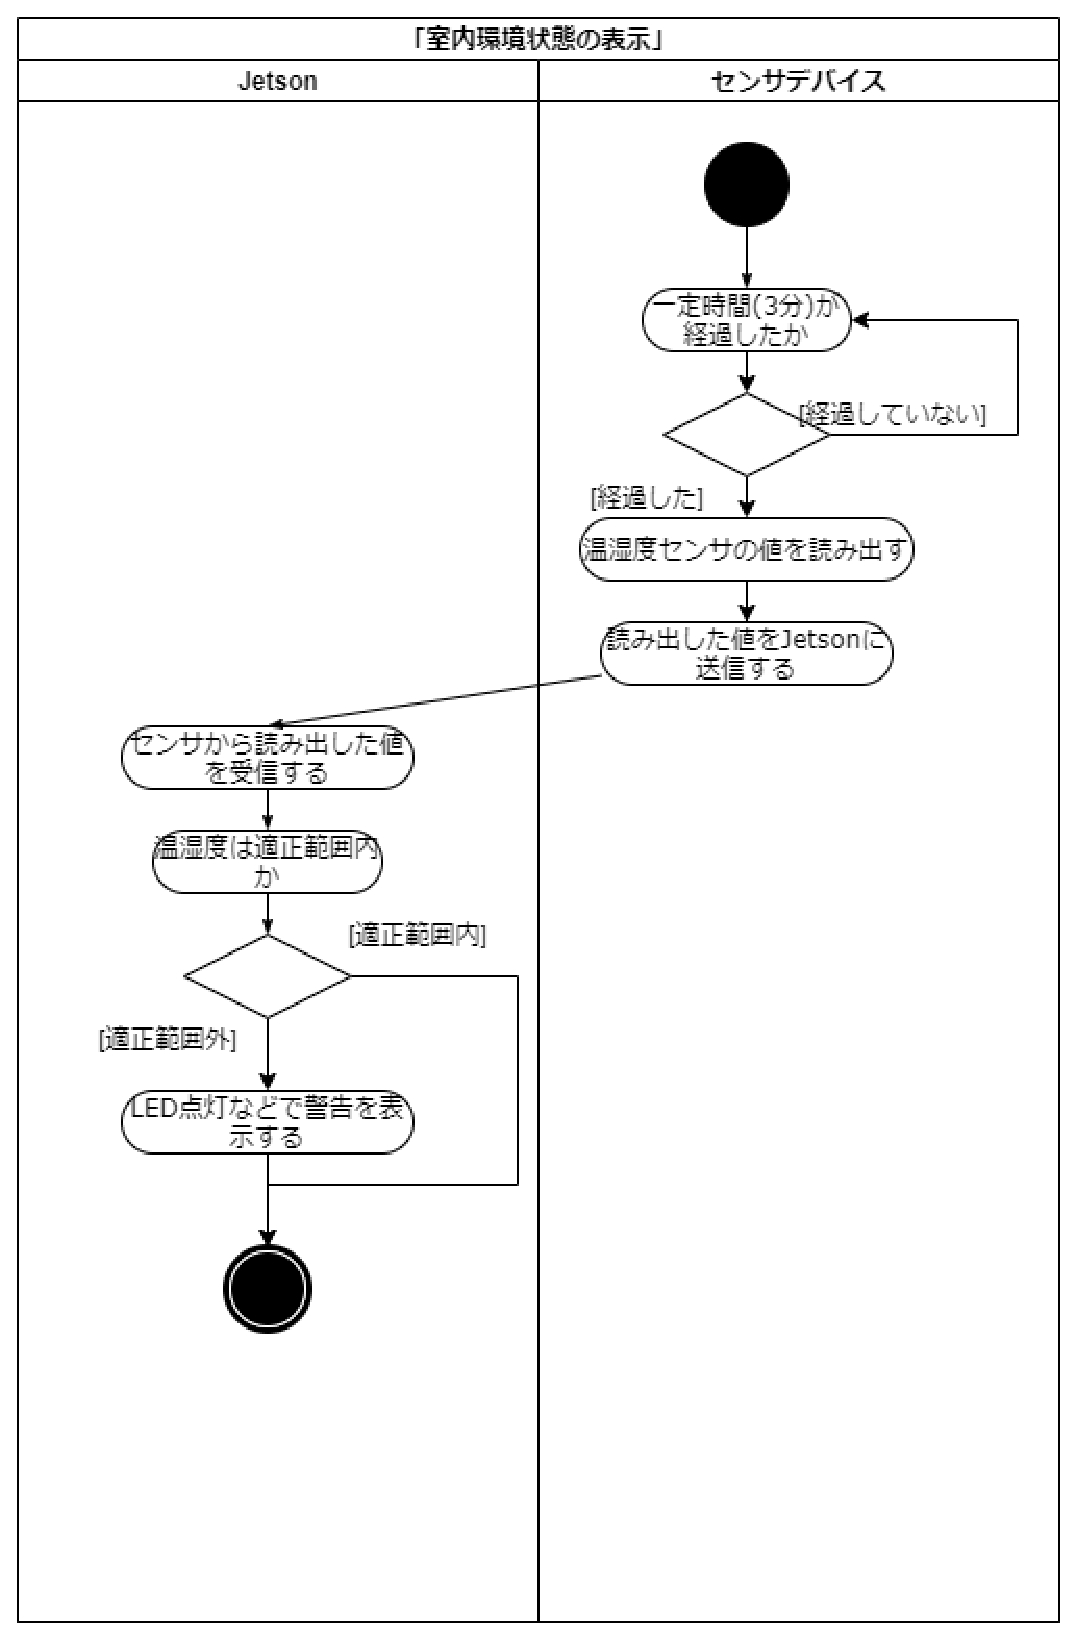
\includegraphics[width=10cm]{a_situnaikankyou.eps}
	\caption{室内環境状態の表示}
	\label{a_situnaikankyou}
\end{figure}

以上の4つのアクティビティ図の作成を通して、それぞれのユースケースを実現する際の処理の流れを可視化することができた。この作業を通して、ユースケース図やユースケース記述を作成した時点よりも、より論理的にシステム内部の設計を進めることができた。

上に示したアクティビティ図では、各デバイスなどのオブジェクトごとの処理のまとまりを、縦の線によってレーンとして明示的に分けて表現している。これによって、各ユースケースの全体的な処理の流れだけでなく、各ユースケースにおいて、処理やデータがオブジェクト間でどのように移されるかを確認することもできた。

具体的に見てみると、室内の複数箇所に設置するセンサデバイスは、センサから値を取得した後は、送信の機能を基本として動作すればよいことが確認できた。一方、Jetson nano側に着目すると、センサデバイスからのデータの受け取りと、室外の入室危険度表示デバイスへのデータの受け渡しというデータの流れが必要となることが確認され、Jetson nano側ではデータの送受信両方の役割を持たせなければならないことが確認できた。また、室外の入室危険度表示デバイス側は、データの取得・分析後の成果物の情報といえる、入室危険度の受け取りさえできればよいということから、受信の機能を基本として動作すればよいことを確認することができた。

アクティビティ図作成の段階では、まだ詳細な処理の流れが示されていないものの、ユースケースを実現する際の大まかな処理とデータの流れを確認することができた。また、この後の詳細設計を進める際にも、ここで作成したアクティビティ図が、基本的な考え方として活かされた。

基本設計の段階では、各デバイスがどのような振る舞いをするかを確認することができたことで、実際にシステムに用いるデバイス類の選定が可能となった。ここまでに、人数推定の機能をリアルタイム性の高い物体検出によって実現するという点から、エッジサーバ側にはJetson nanoを用いることが決まっていたが、この段階でセンサデバイス、室外の入室危険度表示デバイスに用いるデバイス類を決定した。

3.1節でも述べたが、センサデバイスは室内の複数個所に設置することを想定しており、電源の供給方法による取り付け場所の制約を受けず、なおかつ比較的低い消費電力での稼働を可能とするデバイスを選ぶ必要があった。このことから単4乾電池2本で動作し、ワイヤレスセンサーネットワークの構築に適した無線規格であるIEEE802.15.4を採用し、低消費電力での無線通信を可能にする無線マイコンモジュールとしてTWELITEを選定し、室外に設置する部屋への入室の危険度を表示するデバイスに関しても、同じくTWELITEを選定した。また、Jetson nanoにもこのTWE-LITEをUARTによって接続し、センサデバイスとしてのTWE-LITEや、室外の入室危険度表示デバイスとしてのTWE-LITEそれぞれとの通信を可能とし、エッジサーバとして必要となる、データ送受信の機能を持たせている。

ここまでの設計内容をもとにクラス図を作成したところ、図\ref{class}のように本システムの静的な構造が確認できた。ただし、3.4節でも述べるがJetson nano側では、センサデバイスから受け取ったデータを管理するために、データベースを用いることとしている。

\begin{figure}[H]
	\centering
	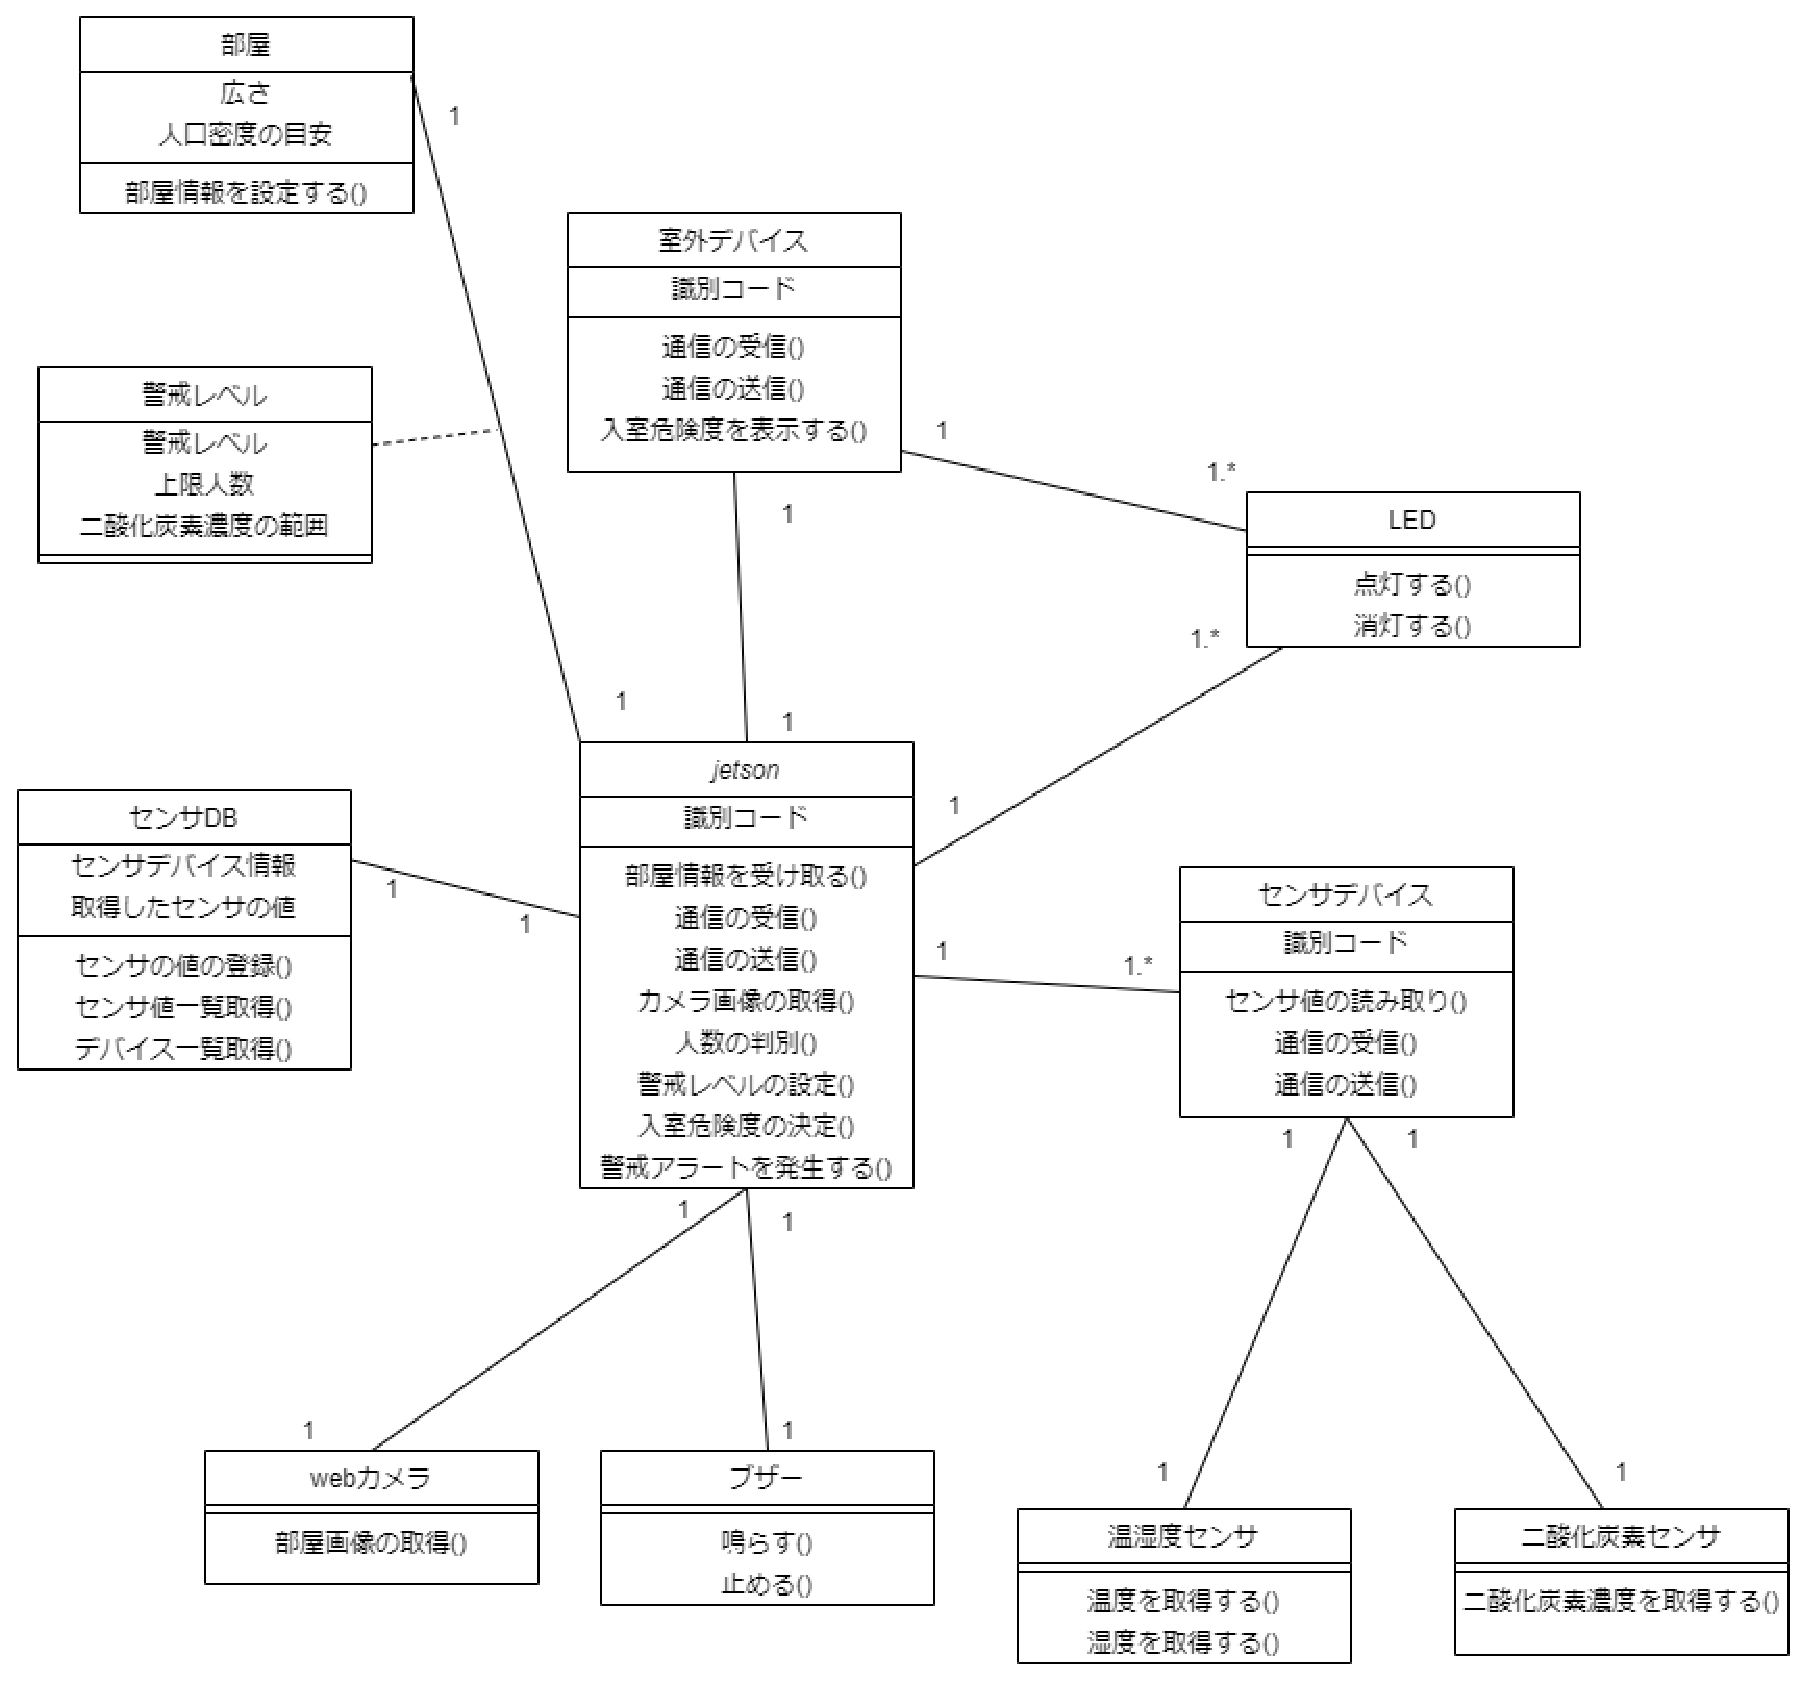
\includegraphics[width=12cm]{class.eps}
	\caption{クラス図}
	\label{class}
\end{figure}


また、以上の基本設計の内容をもとに、結合テスト項目として表\ref{ketugoutest_koumoku}の項目を挙げた。


\begin{table}[H]
	\centering
	\caption{結合テスト項目}
	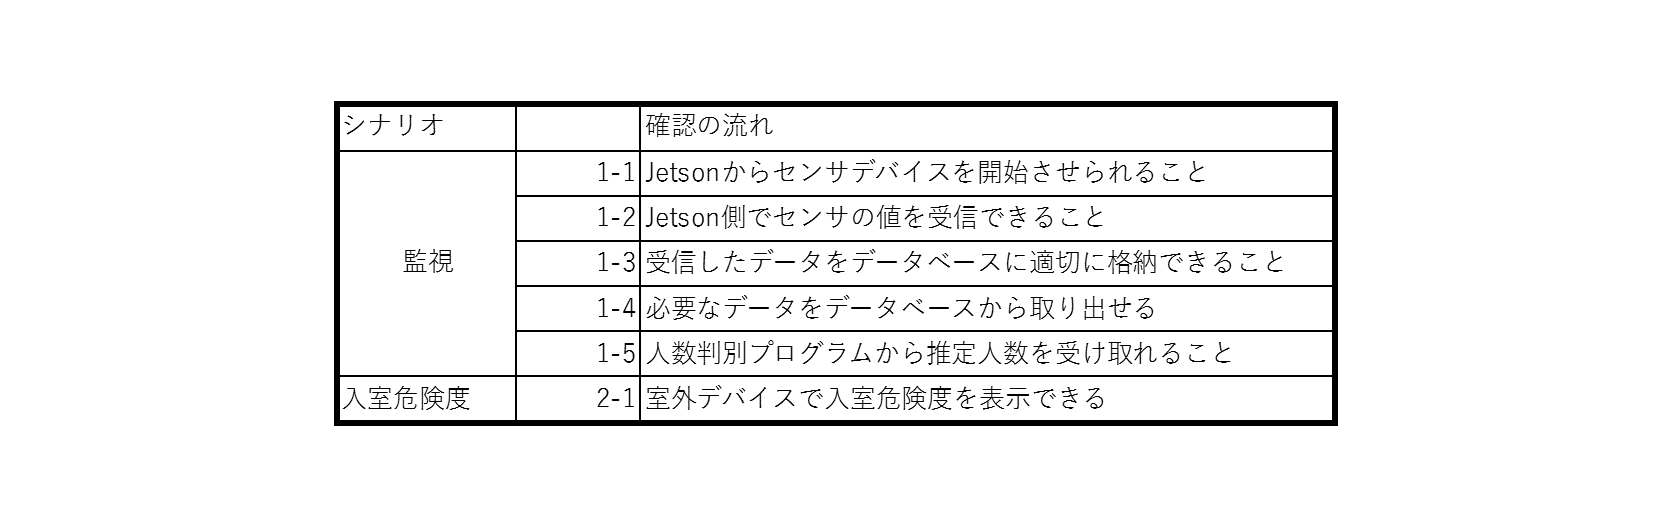
\includegraphics[width=15cm]{ketugoutest_koumoku.eps}
	\label{ketugoutest_koumoku}
\end{table}



